\section{Valeur, direction et sens (3 points)}

On a représenté ci-dessous, les vitesses de 4 objets (A, B, C et D) à un moment précis.

\begin{center}
	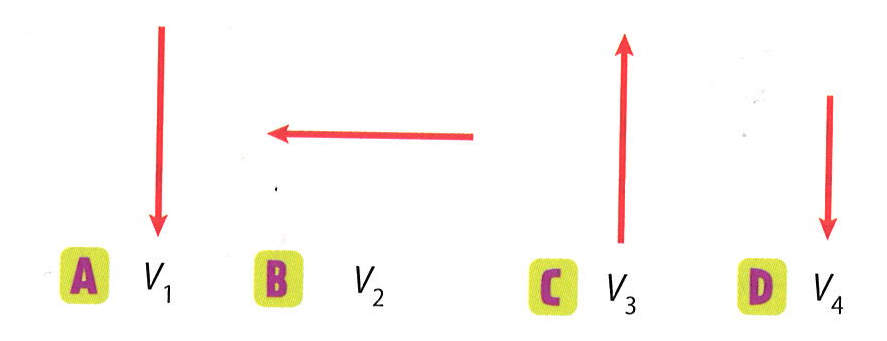
\includegraphics[scale=0.4]{exemples}
\end{center}

\begin{questions}
	\question \'A l'instant représenté, quels objets ont :
	\begin{parts}
		\part[1] la même direction ?
		%\fillwithdottedlines{1.5cm}
		
		\part[1] le même sens de déplacement ?
		%\fillwithdottedlines{1.5cm}
		
		\part[1] la même valeur ?
		%\fillwithdottedlines{1.5cm}
	\end{parts}

\end{questions}